% Chapter Template

\chapter{Experiments on New Routing algorithms} % Main chapter title

\label{coding}

\lhead{Chapter 2. \emph{New Channel Codings}}

\section{Objectives and Scopes}
In this Chapter we are interested in developing system with adding blocks called \textit{Channel Coding}, it's clear that it must add it before all of signalling blocks of Figure \ref{system3} because the idea of channel coding is just adding some logically redundancy bits to permit to receiver at first to detect errors and then the ability of correction in packets. DASH7 protocol uses a channel codings and our scope is to propose a new channel codings to enhance the performance in terms of bit error rate of system.

In information theory, the noisy-channel coding theorem (Shannon's theorem), establishes for any given degree of noise contamination of a communication channel that it is possible to communicate digital information nearly error-free up to a computable theoretical maximum rate which can be calculated by \ref{shannon} through the channel. The Shannon limit or Shannon \textit{Capacity} of a communications channel is the theoretical maximum information transfer rate of the channel, for a particular noise level (SNR). In equation \ref{shannon} $B$ is the Bandwidth, $C$ channel Capacity and $SNR$ is the Signal to Noise Ratio power. Some people also are interested in $\frac{C}{B}$ which is called Spectral Efficiency (SE) of system. Each time that you appliy an Error Control Coding you will have a smaller SE which causes a smaller Bit Error Rate.  


\begin{equation} \label{shannon}
C = B \times log_{2}(1+SNR)
\end{equation}

Globally In Engineering One of the most important issues and parameters is the time that you want to put for a project or work, actually you can not never separate it from one of your minded parameters, it's the reason which for that in practice we are interested in Power and not just Energy, actually the power means the average energy that you can give to a project over time as job is very important, nor you can say easily i will stay 200 years to do my own project, while the technology is growing exponentially each day. So in this part heavily of calculation in function of processes done in code is very important also, more code is efficient more we have a short time to process calculation, for example in some  simulations we had to wait 3 days to obtain the exact results which I put it to do during the weekends to use more efficient of time. while we were using a 4-core dell processor.  
\section{Payload Packet Coding}
In DASH7 protocol has been previewed as we noted in Table \ref{frame_table} we have 2 parts to code, one is \textit{Payload + CRC} in which Payload comes from upper layers, after encapsulation by data link layer 'CRC' will be added at the end of this packet the second is \textit{header} which contains some information about given payload packet and it's ready to give this frame to physical layer to add syncornization part. In this subsection we will talk about coding of payload and the other will be applied on all this packet (without Syncronization) is Convolutional Channel Codes, in this subsection we will propose a new code \textit{LDPC (Low Density Parity Check)} which are named \textit{Capacity-Approaching Codes} because of their Bit Error Rates curves which are very near to Shannon limit against Convolutional codes and after that we will explain the different used algorithms.     

In first part we introduce the curves of BER and BLER for different Coding in different channel, the next part is to introduce the \textit{LDPC} \& \textit{Convolutional} channel codes and then we explain mathematical equations and ideas of Encoding and Decoding algorithms.
  

\subsection{BLER and BER Curves in Different Channel Models of Different Codings}
The BER vs SNR is the curve of Bit Error Rate against of signal to noise ratio, in digital modulation is 
$\frac{E_{b}}{N0}$ which definitely depends on Modulation and Signal Shaping. it's defined by the number of received error bits in packets, divided by the length of packet with an acceptable statistical of test. It means for watching bit error rate of $10^{-4}$, it should have at least $10^{4}$, actually theoricaly it's correct but in practice for a good immunity for example this error probability we test $10^{5}$ or $4 \times 10^{4}$.
BLER is just a measurements which is used more in higher layers (data link, ...) which means that the number of received errors packet.

Figure \ref{ber} is the bit error rate of coherent demodulation without coding of DASH7 (2-FSK, with index of modulation of 1.8 \& 0.5) which by increasing when $h = 0.5$ is better because the discontinuity of signalling is lesser in this case. We can say that BLER is proper to BER, so from this time we only concentrate on BLER curves, because it is more important in terms of protocols.    

Now figure \ref{bler_coding} shows Block Error Rate of system \ref{system3}, clearly the difference between system with coding convolutional and without coding. You can see also a better curve (green) which is better when we put \textit{Zero Padding}. Actually when we put a known word in the end of coding packet to help the algorithm State Machine steps for Viterbi (Hard Decoding). 

Figures \ref{bler_conv} and \ref{LDPC_Conv_final} are the competitions between LDPC and Convolutional coding, Figure \ref{LDPC_Conv_final} shows BLERs figures where LDPC starts to catch Convolutional codes which for \textit{Soft} decoding is about 4.2 dB and for \textit{Hard} decoding is about 5.2. Hard and Soft decoding for LDPC means 'Bit flipping' \& 'Log-Sum Product' and for Convolutional means 'Hard','Soft' decision of Viterbi algorithm. Details of algorithms will be discuessed in future subsection. In all figures packet bits test was for 16 Bytes (128 bits).   

In figure \ref{bler_conv} you can see there are 2 models of channel AWGN which is famous case of just added randomly noise to the transmitted signal and the second is TU5 which is a model of channel used in GSM system for 'Typical Urban' and is implemented by Jakes algorithms in Octave and figure \ref{LDPC_Conv_final} is in TU5 model channel \cite{urban}.

\begin{figure}[h]
\centering
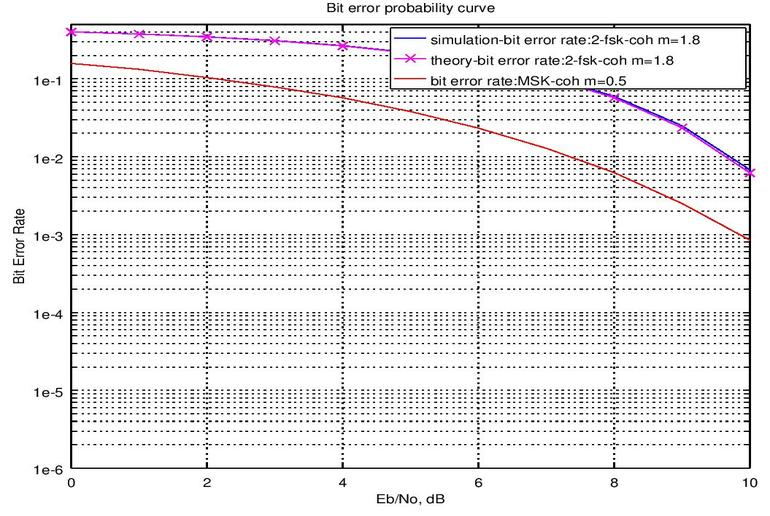
\includegraphics[scale=0.8]{Figures/ber.jpg}
\caption{Bit Error Rate, 2-FSK modulation theory and simulation}
\label{ber}
\end{figure}


\begin{figure}[h]
\centering
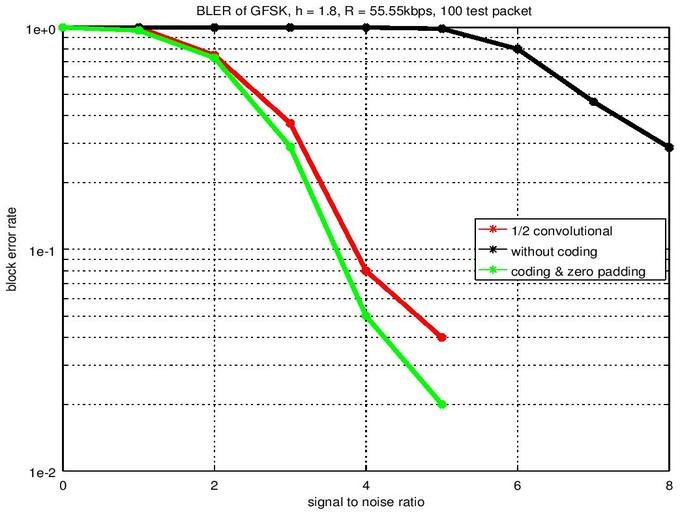
\includegraphics[scale=0.9]{Figures/bler_coding.jpg}
\caption{BLER, with \& without Coding, Zero Padding}
\label{bler_coding}
\end{figure}


\begin{figure}[h]
\centering
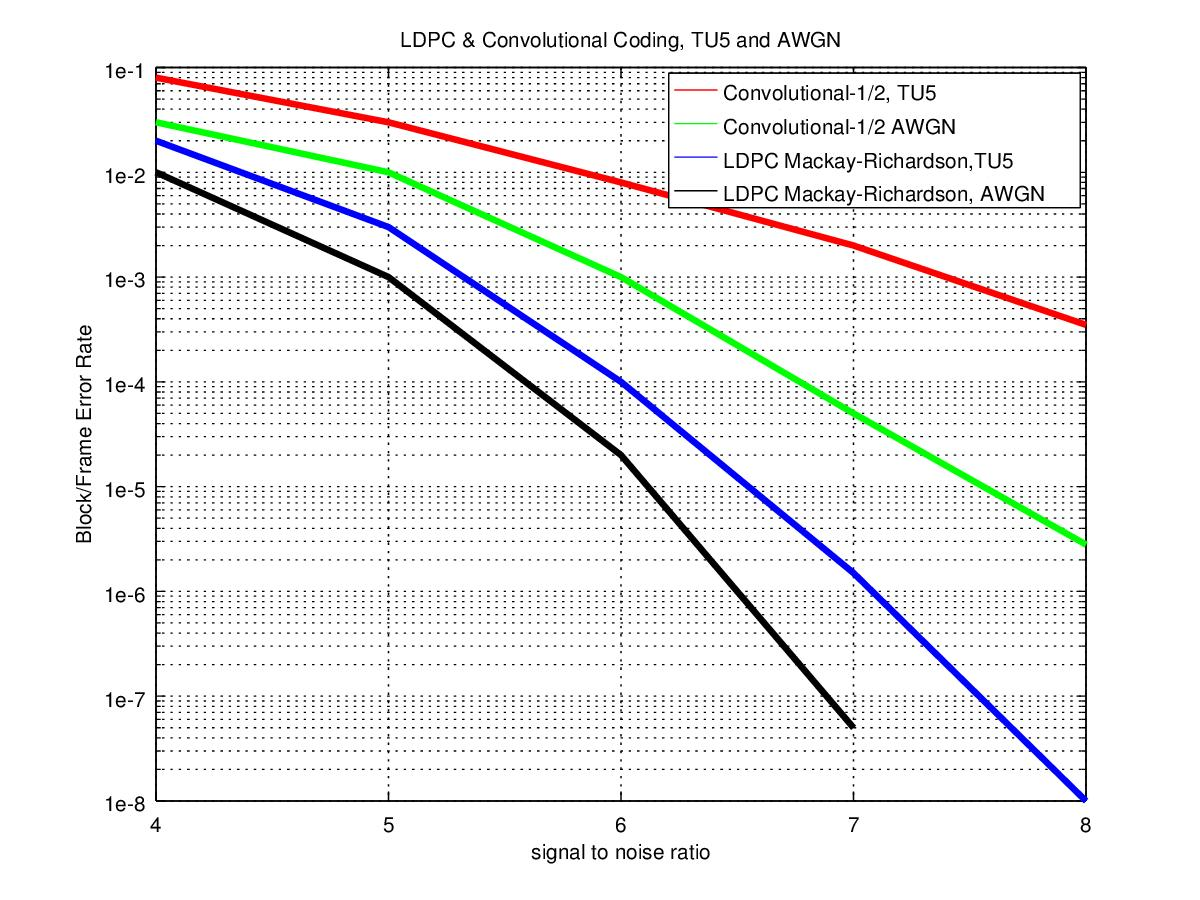
\includegraphics[scale=0.6]{Figures/bler_conv.jpg}
\caption{LDPC(256,128) and Convolutional in AWGN \& TU5 channel model}
\label{bler_conv}
\end{figure}

\begin{figure}[h]
\centering
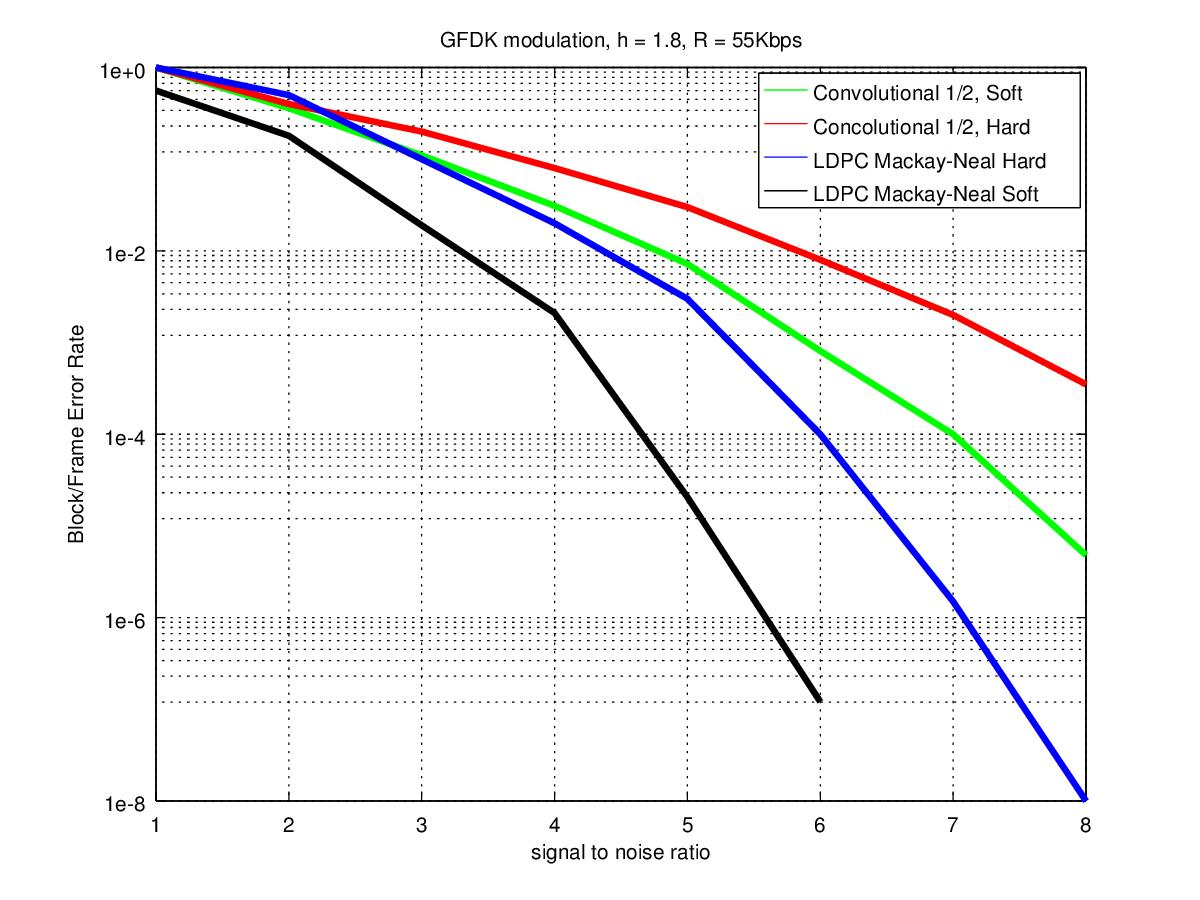
\includegraphics[scale=0.6]{Figures/LDPC_Conv_final.jpg}
\caption{BLER of LDPC(256,128) vs Convolutional Coding with Hard and Soft decoding}
\label{LDPC_Conv_final}
\end{figure}
   
\subsection{LDPC and Convolutional Codes}
In this subsection we are going to explain problems with theoretical and mathematical description.
Globally Error Control Codes are divided by 2 parts 'Convolutional' and 'Block Linear' codes.

Now we are interested in presenting our new channel coding, \textbf{LDPC} codes, which are very high performance and have strong results in Bit Error Rate curves.

Historically, these codes first developed by Gallager in 1963, and then were forgotten until his work was rediscovered in 1996, Turbo codes, another important class of capacity-approaching codes discovered in 1993, became the coding scheme of choice in the late 1990s, used for applications such as the Deep Space Network and satellite communications, but in the last few years, the advances in Low-Density Parity-Check codes have seen them surpass turbo codes in terms of error floor and performance in the higher code rate range, leaving turbo codes better suited for the lower code rates only. 

In 2003, an irregular LDPC code beats six turbo codes to become the error correcting code in the new DVB-S2 standard for the satellite transmission of digital television. The DVB-S2 selection committee made decoder complexity estimates for the Turbo Code proposals using a much less efficient serial decoder architecture rather than a parallel decoder architecture. This forced the Turbo Code proposals to use frame sizes on the order of one half the frame size of the LDPC proposals.

In 2008, LDPC beat convolutional turbo codes as the forward error correction (FEC) system for the ITU-T standard.
G.hn chose LDPC codes instead of turbo codes because of their lower decoding complexity because the proposed turbo codes exhibited a significant error floor at the desired range of operation. LDPC codes are also used for 10GBase-T Ethernet, which sends data at 10 Gigabits per second over twisted-pair cables. In 2009, LDPC codes are also part of the Wi-Fi, 802.11 standard as an optional part of 802.11n and 802.11ac, in the High Throughput PHY specification.
These interests ,volunteers and reasons in LDPC codes caused to think about these codes for DASH7.

The main idea of \textit{LDPC (Low Density Parity Check)} is to produce a parity check matrix which are typically Low Density, means that the number of '1's bit are very smaller than '0's (0.001). It's the reason that codes are very practical for registering datas we need only to register '1's. there are many methods to construct LDPC codes such Gallagar, Prototype, Mackay Neal, Finite Geometry, RS based, Irregular, Random, ... .

In this internship we have tested the easiest to implement (gallagar, Regular, Mackay  Neal) because of practical objectives of internship and we chose Mackay Neal because of Figure \ref{ber_ldpc} which has gotten from \ref{Bibliography}, which is Bit Error Rate of 4 different codes, \textit{Rate 1/2 64 state convolutional}, \textit{Computer generated}, \textit{Mackay Neal} and \textit{EG-Gallagar} which can be concluded the best compromise between these codes, EG-Gallagar and Mackay Neal codes are the best performance in BPSK modulation in AWGN channel. Implementation of EG-Gallagar is difficult in practice. In contrast Mackay Neal codes are near to these codes and are more practical. So we chose Mackay Neal method to construct Parity Check matrix. LDPC codes are introduced using a sparse \textit{bipartite} Graph specially in Designing and Decoding Techniques\citep{errorcontrolcoding}.
    

\begin{figure}[h]
\centering
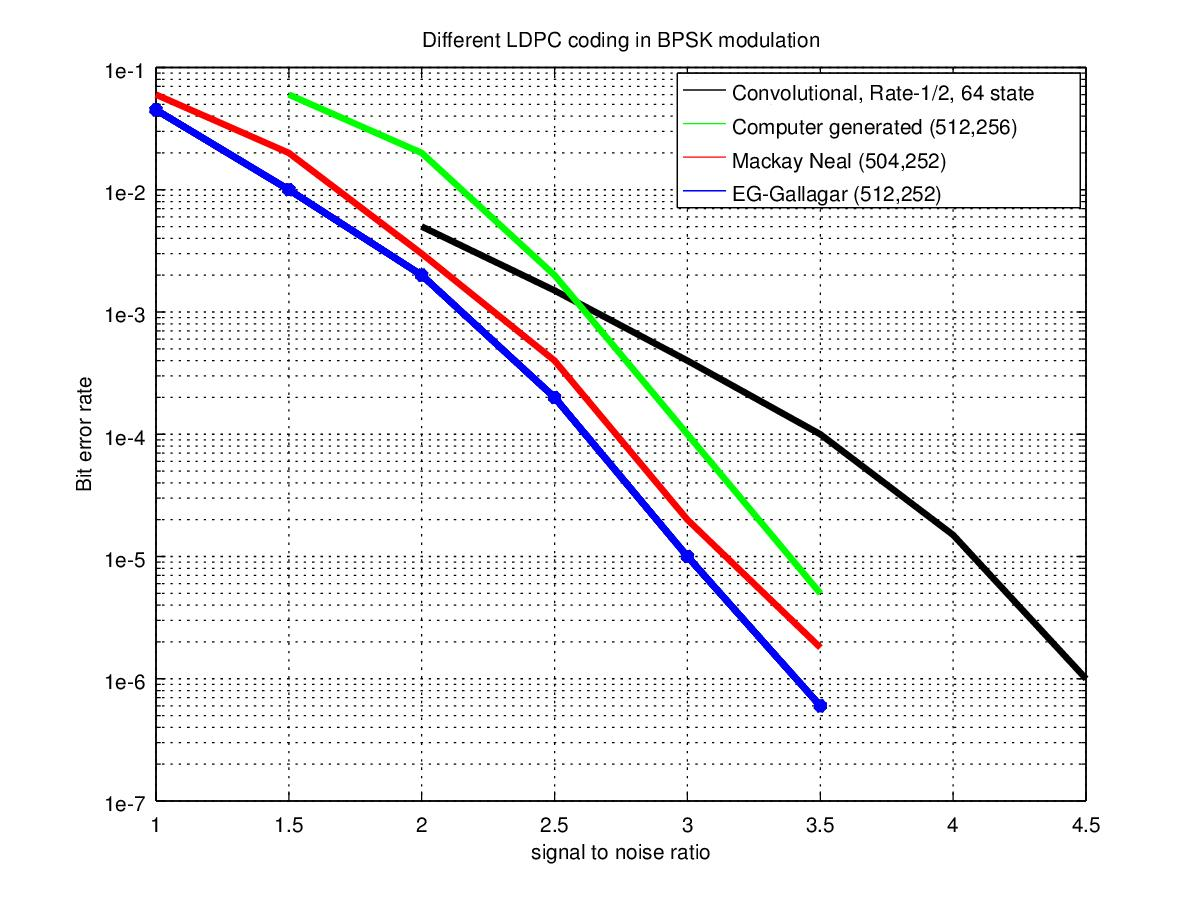
\includegraphics[scale=0.6]{Figures/ber_ldpc.jpg}
\caption{Rate-1/2 64 state Convolutional code, EG-Gallagar (512,256), Mackay Neal (504,252), Computer generated (512,252)}
\label{ber_ldpc}
\end{figure}



\textbf{Convolutional} codes are produced by shift registers which is actually a finite state machine and in function of states and input the output (binary coded) will be produced and  it's very useful and common in practice. Convolutional code used in DASH7 has a rate of 1/2, 3 shift registers with $G(D) = [\frac{D^3+D+1}{D^3+D^2+D+1},\ 1]$ matrix of generator which each $D$ is just an agent of a shift register and 1 is just moment input bit, 2 arguments is because of rate which means that it transforms each bit to 2 bit. Mathematical description let's say if you want to code a given bit for first output of Coding it's just enough to add (in $GF(2)$) all of the register's bits and the input bit and for second output is just enough to add the 3th, second and own bit input to have the 2 bits coded of your suitable bit.  

\textbf{Linear Block Codes}. The  general idea of these codes is to create a linear function (matrix) of binary bits which are basically produced by algebric structure and algebra abstract concepts which own-self obtained by algebric polynomials. These codes have 2 matrix, \textit{Generator}($G$), \textit{Parity Check}($H$) matrices. Generator matrix is a $k \times n$ matrix which $k$ is the number of message bits and $n$ is the length of coded binary stream just a matrix that you can multiply your binary stream and the results is the coded binary stream. There are different methods for Decoding of 'Block linear codes' one can be syndrome decoding algorithm. Actually Parity Check matrix  ($ (n-k) \times n$)permits us to understand if a binary stream is in codeword dictionary. We can check it by this method: Multiplying received bit stream by Parity Check matrix the result is called syndrome of stream. Syndrome is going to check, zero if there is no error in stream and if not by checking this stream in look-up table we can find the proper errors. In which look-up table is the correctable errors.



\subsubsection{Algorithms of Encoding}
\textbf{Algorithm of Encoding of convolutional} coding is by a 3 state memory shift register. The circuit is shown in Figure \ref{conv_block} which just transforms each bit to 2 bits depends on last moment state and input now, equations of matrix generator produce the coded message $G(D)$ form a feedback in practice to be stable so they are usually normalized.

\begin{figure}[h]
\begin{center}
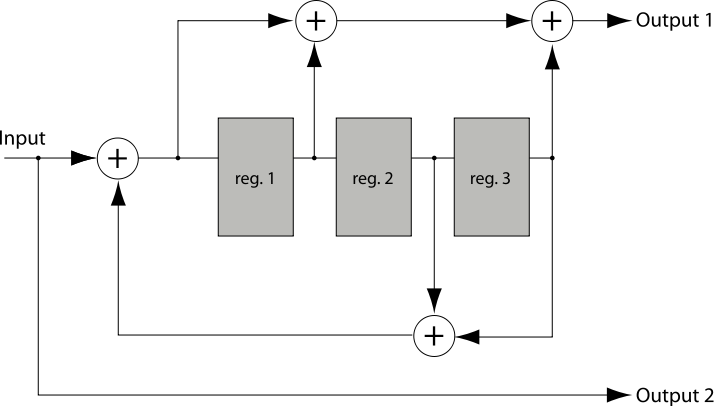
\includegraphics[scale=0.4]{Figures/encoder.png}
\end{center}
\caption{Logical Circuit of DASH7 Convolutional code}
\label{conv_block}
\end{figure}


Actually as we said encoding of linear blocks codes are done by a matrix generator called ($G$) which is just simply a multiplication, the other hand, basically constructing LDPC codes are done by Parity Check Matrix ($H$, which are low density), the problem is for encoding it must transform $H$ to $G$, actually this procedure is not easy, specially when dimensions of parity check matrix is large. In my internship because we wanted to code payload and the minimum acceptable of payload was 16 Byte, we have chosen a parity matrix of 128$\times$256, which means that the rate of coding is $\frac{1}{2}$ and is constructed by \textit{Mackay Neal} method and we have 128 redundant bit for 128 bit message.          

\textbf{Method of Mackay Neal LDPC} is based on producing random columns of $H$ matrix such that there will find no 2 columns or rows as vectors that have maximum in one place the same '1' common. This is because of preventing 4-cycles girth in proper graph The steps of algorithm is this: 1) Producing all zero matrix $M \times N$, 2) In all columns of H and some of rows there will be $\gamma$ bit '1' 3) Become randomly the rows that consists any or just one bit of '1' to 2 bit '1'. 4) In each , $\rho = \frac{N_{\gamma}}{M}$ , must be an integer number if $\rho$ is not an integer, it can not be designed a regular code. 5) If the weight of $ith$ row is greater than $\rho$ randomly  one of the bit '1' of this row is chose and it exchanges with another rows which have a smaller weight against $\rho$, if there is no row by this condition it repeats for the columns. 6) Preventing the 4-cycle path in proper graph.     

There are also another methods which are just the subsection of this algorithm, which can be generated by producing 2 submatrices seperatley cunstructed by LDPC methods.

\textbf{Girth of LDPC}. In LDPC Parity Check matrices there is a parameter called \textit{girth} of matrix, is just a parameter in LDPC codes which demonstrate the degree of ability of code some increasing in girth which progress the performance is basically to prevent 4-cycle in Tanner graph of code. One of the most important challenges in LDPC codes is \textit{Cycle Decomposition}, 4-cycle (vertices of rectangle of bit '1') in $H$ it can be heavily degraded the performance of code.  Bipartite graph of code searches all of equations to be satisfied to be correct or not. Actually for preventing of these 4-cycles we transform each columns or rows of $H$ by 2. This procedure is called \textit{Cycle Decomposition} and we'll have an expanded code in which the cycle of parities check is lesser and it can increase the performance of code. This algorithm prevents these 4-cycles. We have used an \textit{irregular matrix code with $\rho = 3$ \& $\gamma = 6$ are the mean of rows, column's Hamming weight}. In practice Irregular LDPC codes are more useful because of their better performance.

\textbf{Encoding LDPC}. Compared with general linear block codes, LDPC encoding with \textit{Lower Triangular Check Matrix} and \textit{Approximate Lower Triangular Check Matrix} carry out encoding directly by parity check matrix $H$. There are two types of encoding by lower triangular check matrix structure. The first is to use the Gaussian elimination to convert the check matrix H into lower triangular matrix structure before encoding. The encoding complexity is $O(n^{2} )$, $n$ is the column of check matrix. However, lower triangular check matrix produced in this method is not consistent with the sparse characteristics. The second is to directly use a given lower triangular sparse check matrix for encoding, which may result in loss of encoding performance.

Approximate lower triangular LDPC encoding was proposed by Richardson and Urbanke in 2001. The encoding is to disintegrate the check matrix H (as shown in Figure \ref{matrix}) into six ($A, B, C, D, T , E$) sparse sub-matrix before working out the redundant bit $p1$ , $p2$ (Equations \ref{matrixeq}) according to the characteristics of the six sparse sub-matrix to complete the encoding. The encoding complexity is $O(n + g^{2})$, $g$ is the row of matrix $E$. Compared with the lower triangular encoding matrix, the complexity is lower and the encoding is consistent with the sparse characteristics; hence, the encoding performance is relatively higher. Coded message will be $c = [m, p1 ,p2]$.
\begin{figure}[h]
\centering
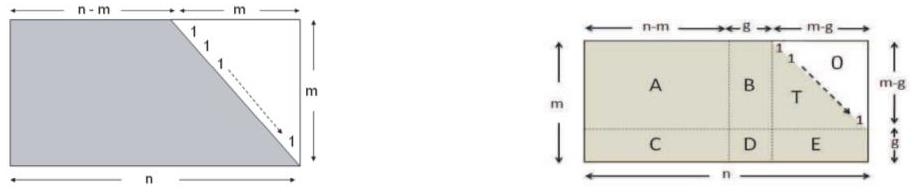
\includegraphics[scale=0.6]{Figures/matrix.jpg}
\caption{Left : Lower Triangular Check Matrix , Right : Approximate Lower Triangular Check Matrix }
\label{matrix}
\end{figure}


 
\begin{equation} \label{matrixeq}
\left\{\begin{matrix}
Am + Bp_{1} + Tp_{2} = 0 \\
(-ET^{-1}A + C)m + (-ET^{-1}B + D)p_{1} = 0
\end{matrix}\right.
\end{equation}

\begin{equation}
H = 
\begin{bmatrix}
 & A & B & T\\ 
 & -ET^{-1}A + C & -ET^{-1}B + D & 0
\end{bmatrix}
\end{equation}

Actually algorithm of Richardson-Urbanke has been designed for regular LDPC codes which have a Quasi-Cyclic, Block-Circulant which are more easy to encoding , i tested for irregular LDPC (Smaller Girth-Cycle, more Sparse Parity Check Matrix) and we gave a suitable performance. In Encoding We have registered 6 sub-matrices and it's done by a combination of these matrices to message without using a generator matrix ($G$)\citep{richardson}.  


%\tikzstyle{ann} = [draw=none,fill=none,right]
%%\tikzset{mystyle/.style={draw,circle,label={[fill=yellow]0:#1}}}
%\node [block] (FF1) {FF1};
%\node [block,right =0.5cm of FF1] (FF2) {FF2};
%\node [block,right =0.5cm of FF2] (FF3) {FF3};
%\node [block,below right = 0.5cm and 0.5 cm of FF3]  (c1) {c1};
%\path[draw,->] (FF1) edge (FF2)
%			   (FF2) edge (FF3)
%			   (FF3) edge (c1)				   
%			    ;	




\subsubsection{Algorithms of Decoding  (Hard and Soft decision)}
\textbf{Decoding of Convolutional}. Codes are done normally by a prestigious algorithm called \textit{Viterbi}, which is used in any random Markov process, the idea is to find the shortest path that a binary stream could be coded. Shortest path is measured by a metric called \textit{Euclidean Distance} which is in Galois binary Field ($GF(2)$) or can be in $\mathbb{R}$ numbers and will be produced Hard and Soft decision respectively. Imagine you have a $n$ binary stream to decode, Viterbi algorithm starts from the first bit and calculate all possibilities of coded paths in each steps eliminates the paths that are larger value of metric, simply because of Maximum likelihood concept and at the end you will have your most probably path which have should be received.

\begin{figure}[htbp]
\centering
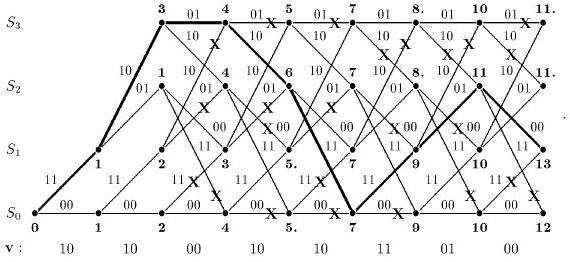
\includegraphics[scale=0.6]{Figures/viterbi.jpg}
\caption[Viterbi decoder, $R = \frac{1}{2}, K = 3$, BSC channel]{Viterbi decoder, $R = \frac{1}{2}, K = 3$, BSC channel}
\label{viterbi}
\end{figure}

Normally Viterbi algorithm is done by \textit{Trellis} graph (Figure \ref{viterbi}), in which you can see the time effect and elimination of less probable paths on algorithm. If before of decision we apply received analogue signal to Viterbi somehow we will have an effectively non-binary Euclidean Metric result will be more correct which approximately gains 2dB in theory. 
In internship we didn't have access to inside of chips and the bases of chips get binary numbers and it can't get non-binary numbers. 

\textbf{Decoding of LDPC}. Optimum (Maximum Likelihood) decoding of LDPC codes is in general not feasible for the reason of complexities. The algorithm of Viterbi is optimal while generally the algorithms of LDPC codes are suboptimal which are popular because of error probability performance. An LDPC coded can be decoded in various ways, namely: Majority-Logic (MLG), Bit Flipping (BF), Weighted BF (WBF), A Posteriori Probability (APP) and Iteratively Decoding based on Belief Propagation (IDBP) (commonly known as sum-product algorithm (SPA)). The first 2 types are hard decision, the last 2 are soft-decision decoding and the third one is in between. MLG decoding is the simplest one in decoding complexity. BF decoding requires a little more decoding complexity but gives better error performance than the MLG decoding. APP decoding and the SPA decoding provide musch better error performance but require much larger decoding complexity than the MLG and BF decodings. The weighted BF offers a good trade off between error performance and decoding complexity. SPA decoding gives the best error performance among the five types of decoding of LDPC codes and yet is partially implementable. APP decoding also provides the best error performance; however it is computationally intractable and hence will not be considered as a candidate of decoding algorithm\cite{errorcontrolcoding}. These reasons make us to choose \textit{Bit Flipping} (Figure \ref{bipartite}) for hard decoding and \textit{Log-Domain SPA} (an implementable version of SPA) proposed by \cite{logdomain} for soft decoding. We explain now these algorithms in more details

%
\begin{figure}[htbp]
\centering
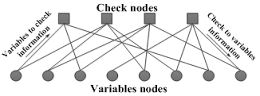
\includegraphics[scale=0.8]{bipartite.png}
\caption[Bipartite Graph Demonstration for Decoding]{Bipartite Graph Demonstration for Decoding}
\label{bipartite}
\end{figure}

%
Algorithm of \textit{Bit Flipping} is done by this steps with Equations of \ref{bitflipping} in which, $z$ is the \textbf{Hard} decision , $H$ parity check matrix and $\textbf{s}$ syndrome of received signal. The steps of algorithm is below :

1) compute the parity check sums (syndrome bits) based on \ref{bitflipping}, if all the parity-check sums are zero, stop the decoding. 2) Find the number of failed parity check equations for each bit, denoted by $f_{i}, i =0,1,..., n-1$. 3) Identify the set $\mathbb{S}$ of bits for which f$_{i}$ is the largest. 4) Flip the bits in set $\mathbb{S}$. 5) Repeat steps 1 to 4 until all the parity check sums are zero (for this case, we stop the iteration in step 1) or a maximum number of iterations is reached.)

\begin{equation} \label{bitflipping}
\left\{\begin{matrix}
\textbf{s} = (s_{1},s_{2}, ..., s_{J}) = z . \textbf{H}^{T} \\
s_{j} = \textbf{z} . \textbf{h}_{j} = \sum_{l=0}^{n-1} z_{l}h_{j,l}\\
\textbf{h}_{j} = (h_{j,0},h_{j,1}, ...,h_{j,n-1})
\end{matrix}\right.
\end{equation}
%

\textbf{Soft} decoding is done by \textit{Log-Domain SPA} which is just a SPA using Log-Likelihood-Ratio (LLR- A posteriori probability) metric to measure the equations of normal-SPA and is done by these steps:

1) Initialization step: variable nodes are initialized with the belief of the corresponding variable, based solely on the received vector $x$. 2) Tentative decoding: variable node n computes, based on all the information it has available (i.e from the channel vector x and messages from adjacent check nodes), the most likely value of the variable $n$, $c_{n}$. If the decoded nodes satisfies all checks ($\textbf{H . c} = 0$), the  decoding algorithm is halted. 3) Horizontal step: a message denoted is passed from variable node $n$ to check node $m$. expressing the belief of the $nth$ variable, given all the information from all connected check nodes, except check node $m$ itself. 4) Vertical step: each check node $m$ sends a message to adjacent variable node $n$, reflecting the belief of the $nth$ given all the information from the channel and all variable nodes connected to check node $m$, except variable $n$ itself. Go to step (2). Effectively in this procedure $z$ of first equations \ref{bitflipping}  is the received signal before applying hard decision \citep{errorcontrolcoding} \cite{LDPC}.

\subsection{Cyclic Redundancy Check Codes (CRC)}
This family of Error Control Codes belongs to the family of \textit{Detecting} error control codes actually there is a lot of kinds of this family like : CRC-8, CRC-16, CRC-32, CRC-64, Checksums algorithms and ... . Actually DASH7 uses CRC-16 ITT of this family and actually in data linke layer when a packet comes down, this layer is going to encapsulate this packet and make a frame by this way that it adds a 'header' at first of packet and a \textit{CRC} part at the end of frame which contains 16 bits.
 In the receiver frame is checked and if the packet is not a good version it will send the No acknowledgement to sender to retransmit it again. Mathematical equation is given in \ref{crc}:
 
 \begin{equation}\label{crc}
g(x) = x^{16}+x^{12}+x^{5}+1
\end{equation}

As for note, Frame/Block Error Rate is a criteria measuring in data link layer of network, it means that if you want to measure your quality of service in this layer, theoretically because the bits have been framed   
 so the smallest piece is the \textit{frame}, by checking the error occurred inside frame you can define your criteria against energy which is Frame Error Rate. in Figure \ref{LDPC_crc} you can find final coding Frame Error Rate of payload packet (\textit{LDPC + CRC}). 
 
 \begin{figure}[htbp]
\centering
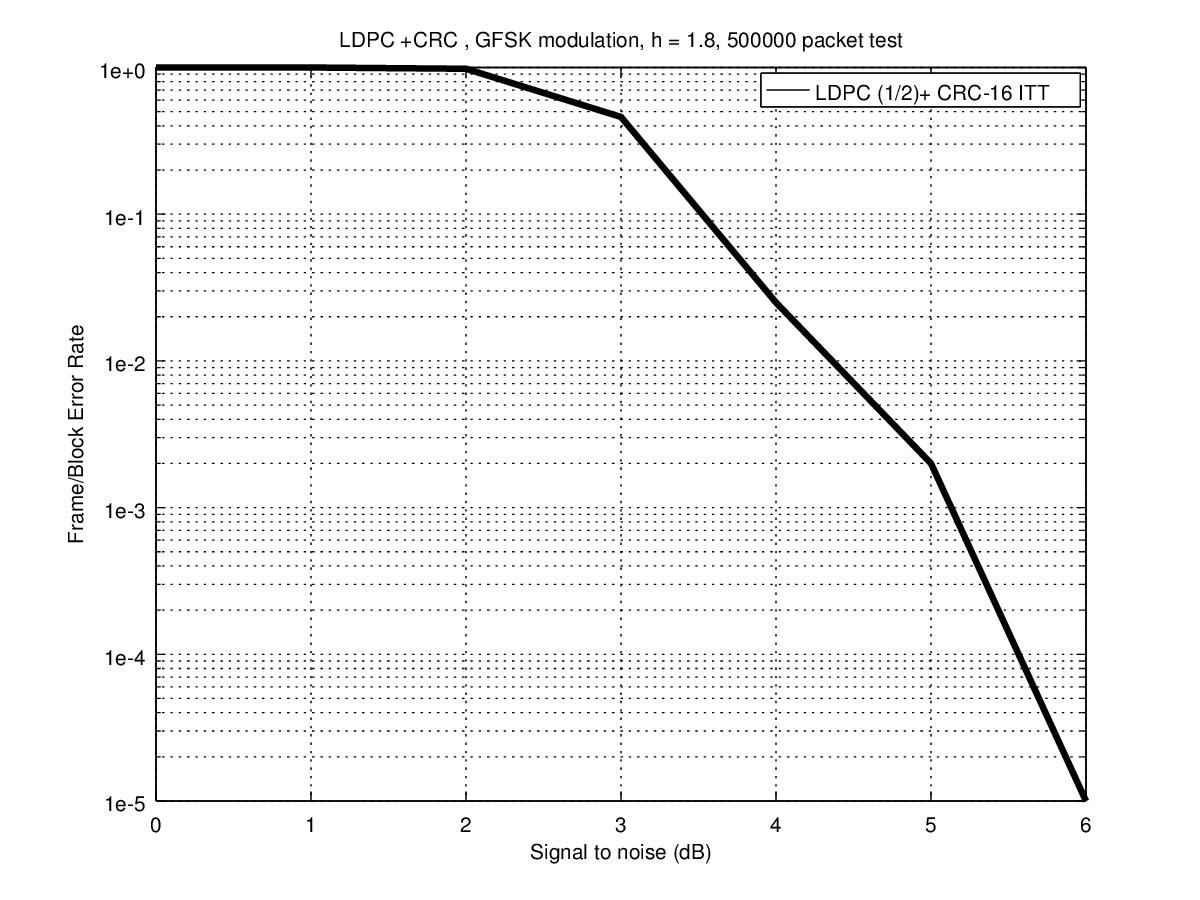
\includegraphics[scale=0.6]{Figures/ldpc_crc.jpg}
\caption[LDPC(256,128) + CRC16-ITT]{LDPC(256,128) + CRC16-ITT Frame Error Rate}
\label{LDPC_crc}
\end{figure}

 
%
\section{Header Packet Coding}
As it is mentioned in Table \ref{frame_table} from Chapter \ref{dash7} we will apply a special channel coding on head of packet, so in parallel and we will propose 2 channel coding, generally channel codes are designed for detecting and correcting bits.

In DASH7 header consists of 28 bits which are some datas about the packet (128 bits payloads) which comes from upper layer as it has been well explained and in this way if we would design a code which could well correctly decode in receiver we will Header of packet and we will sure about header information.


\subsection{BLER Curves of Reed-Solomon and LDPC}

The point is in (BER vs SNR) figures the gradient of LDPC codes are fast and they are very near to their Shannon limit but also RS codes give good performance and fast slopes we can design a RS code which for a fixed arbitrary error probability because the gain of coding is a function of Bit/Block Error Probability. Figure \ref{rs} shows an RS code which satisfies this condition.


\begin{figure}[htbp]
\centering
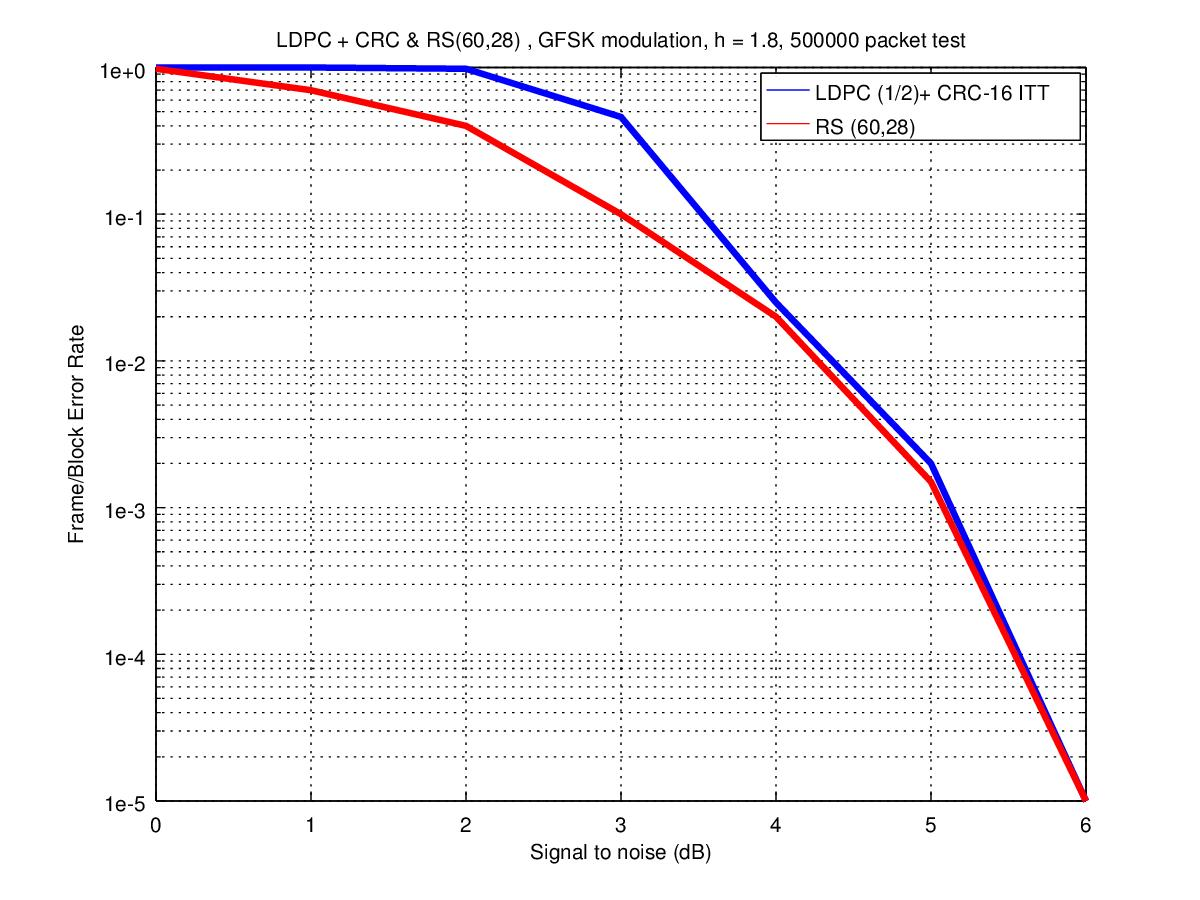
\includegraphics[scale=0.6]{Figures/LDPC_RS.jpg}
\caption[LDPC vs RS code BLER]{BLER of (LDPC(256,128) + CRC-16ITT) and RS(60,28)}
\label{rs}
\end{figure}


\subsection{Reed-Solomon encoding and decoding algorithms}
RS codes are one of the most important codes, extended of BCH codes in which the coefficient of generator polynomials can be in $GF(q)$ and in general form they have Equation \ref{rspoly} in which $t$ is the number of correctable bit in code, $\alpha^{i}$ is the roots of extended binary Galois Field, $GF(2^{m})$ which are made up by primitive polynomials. In this case $m = 4$ which codes 7 bit to 15 bit so the rate of code is $\frac{7}{15}$ and in desired region works we want. RS codes can achieve the maximum value of $d_{min}$ (minimum Hamming distance in code words) which is $n-k+1 = 2t - 1$ in which $n$ is the length of number coded, $k$ is the length of message, $t$ is the number of ability of correction errors. This code is very useful in the 'Burst' Errors which is the case of fading channels the other hand some applications like IEEE 802.16 Broadband Wireless communication they use a combination of this codes with convolutional codes with block of Interleaving and will give very good performances.

 \textbf{RS Coding} We can use algebric appearances of these codes and multiplication message into generator polynomial, coded message will be obtained. Algebric mathematical method permit to write these codes in form of Equation \ref{awgnrs}
 
\textbf{RS Decoding} Main algorithms of RS decoding are \textit{Error Trapping \& Berlekamp-Massey}. Berlekamp-Massey uses some matrix calculation and so it will have heavily calculation of matrix. Error Trapping is a good algorithm specially in practice because it's very compatible with shift Registers and steps of algorithms are done by registers. The idea is division polynomials until the Hamming weight of residual would be equal to the number of correctable bits ($t$)\citep{rs}. 

An example  can be RS(7,3;5) ($n = 7,k = 3, d_{min} = 5$) with generator polynomial of $g(x) = 1+\alpha^{4}x+\alpha^{2}x^{2}+\alpha^{4}x^{3}+x^{4}$ in $GF(2^{3}) = \lbrace0,1,\alpha,\alpha^{2},\alpha^{3} = \alpha + 1,\alpha^{4} = \alpha^{2}+\alpha,\alpha^{5}= \alpha^{2}+\alpha+ 1, \alpha^{6}= \alpha^{2}+ 1\rbrace$ in basis polynomial of $p(x) = 1 +x +x^{3}$   which is seen $e(x) = x^{3}+x^{2}$. Steps of error trapping is shown which is used in decoding algorithm ,below for this example:

\begin{tabular}{c|c|c|c|c|c|c|c}
$v(x)$  & 1 & 1 & 1 & 1 & 1 & 1 & 1\\
$e(x)$  &  0 & 0 & 1 & 1 & 0 & 0 & 0\\ \hline 
$r(x)$  &  1 & 1 & 0 & 0 & 1 & 1 & 1\\ 
$g(x)$  &  1 & $\alpha^{4}$ & $\alpha^{2}$ & 1 & 0 & 1 & $\alpha^{5}$\\ \hline
  & 0 & $\alpha^{5}$ & $\alpha^{2}$ & $\alpha^{4}$ & 0 & 1 & 1 \\
$\alpha^{5}g(x)$ &  & $\alpha^{5}$ & $\alpha^{2}$ & 1 & $\alpha^{2}$ & $\alpha^{5}$ & \\  \hline
  & 0 & 0 & 0 & $\alpha^{5}$ & $\alpha^{2}$ & $\alpha^{4}$ & 1 \\  
$\alpha^{5}g(x)$ & $\alpha^{5}$ & & & $\alpha^{5}$ & $\alpha^{2}$ & 1 & $\alpha^{2}$\\ \hline
 & $\alpha^{5}$ & 0 & 0 & 0 & 0 $\alpha^{5}$ & $\alpha^{6}$ \\
 $\alpha^{5}g(x)$ & 1 & $\alpha^{2}$ & $\alpha^{5}$ & 0 & 0 & $\alpha^{5}$ & $\alpha^{2}$\\ \hline
  & $\alpha^{4}$ & $\alpha^{2}$ & $\alpha^{5}$ & 0 & 0 & 0 & 1 \\
 $g(x)$ & $\alpha^{4}$ & $\alpha^{2}$ & $\alpha^{4}$ & 1 & 0 & 0 & 1\\ \hline   
  & 0 & 0 & 1 & 1 & 0 & 0 & 0\\ 
\end{tabular}
 
- In each steps buffer shifts generator polynomial circulant ($i$) by $\alpha^{i}$ multiplication to get the desired result. 

\begin{equation}\label{rspoly}
g(x) = \prod_{i=1}^{2t} (x-\alpha^{i})
\end{equation}

\begin{equation}\label{awgnrs}
 r(x) = m(x) g(x) + e(x) 
\end{equation}      

Other algorithm, 'Berlekamp-Massey' is a useful computer implementable algorithm by follow:
%
1)Calculate of syndromes vectors $S_{1},S_{1}, ...,S_{2t}$ by equation of \ref{berlekamp}.

2) Initializing algorithm by $k = 0$, $\Lambda^{(0)}(x) = 1, L = 0, T(x) = x$

3)$k = k +1$, %calculate of $\Delta^{k}$ by equation of \ref{chien} 

4) If $\Lambda^{k} = 0$, jump to (8).

5) Update error place pointer polynomial by equation \ref{lambda}.

6)If $2L\geqslant k$, jump to (8).

7)$L = k - L$, calculate $T(x)$ from equation \ref{tx}

8) $T(x) = xT(x)$.

9) if $k<2t$, jump to (3) 10)roots of $\Lambda(x)$ polynomial are the placement of errors \cite{rs}. 


\begin{equation}\label{berlekamp}
S_{i} = r(\alpha^{i})
\end{equation}

\begin{equation} \label{chien}
\Delta^{k} = S_{k} - \sum_{i = 1}^{L} \Lambda_{i}^{k-1}S_{k-i}
\end{equation} 

\begin{equation} \label{lambda}
\Lambda^{k} (x) = \Lambda^{k-1}(x) - \Lambda^{k} T(x)
\end{equation}

\begin{equation} \label{tx}
T(x) = \frac{\Lambda^{k-1}(x)}{\Lambda^{k}}
\end{equation}


This code can be used in parallel as coding of \textit{Header} to have good performance and to be sure to have ability of correcting header because the information in header determines the length of upper given packets. and by applying LDPC codes on payload of frame we will have a good performance for Error Controlling of DASH7 protocol. 